\section{Abstract}
A model for the solar system using ordinary differential equations was developed with the Velocity Verlet method. The earth sun system, earth sun jupiter system and the whole solar system was examined.


\section{Introduction}
In this project I will develop a model simulating the solar system using a set of ordinary differential equations based on Newton's laws of motion:

$\frac{d^2x}{dt^2} = \frac{F_{G,x}}{M_{earth}}$\\

$\frac{d^2y}{dt^2} = \frac{F_{G,y}}{M_{earth}}$\\

$\frac{d^2y}{dt^2} = \frac{F_{G,z}}{M_{earth}}$\\

$F_{G,x}$ = $\frac{-GM_{\odot}M_{earth}}{r^2}cos\theta sin\psi$= $\frac{-GM_{\odot}M_{earth}}{r^3}x$\\

and\\

$F_{G,y}$ = $\frac{-GM_{\odot}M_{earth}}{r^2}sin\theta sin\psi$= $\frac{-GM_{\odot}M_{earth}}{r^3}y$\\

similarly\\

$F_{G,z}$ = $\frac{-GM_{\odot}M_{earth}}{r^2}cos\psi$= $\frac{-GM_{\odot}M_{earth}}{r^3}z$\\


Numerical methods will be used to solve these equations. An initial test for various methods include the Forward Euler, Central Euler and the velocity Verlet methods. For the complete system the velocity Verlet method will be used.\\


In the process of ending up with a solar system I will start by considering basic interaction between the Earth and Sun, before expanding the model to a 3-body problem involving Jupiter, and finally including all planets of the solar system. 





\section{Methods}
%*Formalism/methods: Discussion of the methods used and their basis/suitability. Total number of possible points 20*
\subsection{Forward Euler}
The Euler method tries to calculate an unknown curve starting in a given point satisfying a certain differential equation.\\
\begin{equation}
\frac{dy}{dt}=f(t,y)
\label{Eq:diffeq}
\end{equation}
, where $y(t_0)=y_0$ and $y'(t_0) = v_0$\\


Forward Euler tries to approximate a function curve by a polynomial. The derivative on the left hand side is approximated with a forward step using a Taylor expansion:\\
$y(t+\Delta t) = y(t) + y'(t)\Delta t + O(\Delta t^2)$\\
Neglecting 2nd order terms and higher and solving for y'(t):\\
$y'(t) = \frac{y(t+\Delta t)-y(t)}{\Delta t}$\\
Inserting into equation~\ref{Eq:diffeq} and solving for $y(t+\Delta t)$:\\
$y(t+\Delta t) = y(t)+\Delta t f(t,y(t))$\\


Let $t_n = t_0+n\Delta t$\\


The total solution can be found by iterating from n=0 to n:\\
\begin{equation}
y_{n+1} = y_n+f(t_n, y_n)\Delta t
\label{Eq:Forward_Euler}
\end{equation}\\

\subsection{Central Euler}
Central Euler method approximates the derivative $\frac{dy}{dt}$ with a central approximation:
$\frac{dy}{dt} \approx \frac{y(t+\Delta t) -y(t-\Delta t)}{2\Delta t}$\\

Inserting into equation~\ref{Eq:diffeq} and solving for $y(t+\Delta t)$:\\

$y(t+\Delta t) = y(t-\Delta t)+2\Delta t f(t,y(t))$\\


Let $t_n = t_0+n\Delta t$.\\


The total solution can be found by iterating from n=0 to n:\\
\begin{equation}
y_{n+1} = y_{n-1}+2f(t_n, y_n)\Delta t
\label{Eq:Central_Euler}
\end{equation}\\

Computing $y_1$ at the start of Central Euler iteration is problematic, because it depends on position $y_{-1}$, which is unknown. Therefore in the first step we use the Forward Euler method. The error of the first time step is then of order $O(\Delta t^2)$. This is not considered a problem because the error of the initial value is small compared to the total error accumulated at time $t=t_n$

\subsection{Velocity Verlet}
The Velocity Verlet method uses a central method to approximate the 2nd order derivative. Velocity Verlet method builds on the basic Verlet method:\\

\begin{equation}
\frac{d^2y}{dt^2}=f(t,y)
\label{Eq:diffeq_verlet}
\end{equation}
, where $y(t_0)=y_0$ and $y'(t_0) = v_0$\\



$\frac{d^2y}{dt^2} \approx \frac{y(t+\Delta t) -2y(t)+y(t-\Delta t)}{\Delta t^2}$\\

inserting into equation~\ref{Eq:diffeq_verlet} and solving for $y(t+\Delta t)$:\\

$y(t+\Delta t) = 2y(t)-y(t-\Delta t)+\Delta t^2 f(t,y(t))$\\


Let $t_n = t_0+n\Delta t$.\\

The total solution can be found by iterating from n=0 to n:\\
\begin{equation}
y_{n+1} = 2y_n - y_{n-1} + f(t_n, y_n)\Delta t^2
\label{Eq:Verlet}
\end{equation}\\

Computing $y_2$ at the start of Verlet iteration at n=1, time $t=t_1=\Delta t$, one already needs the position vector $y_1$ at time $t=t_1$. At first sight this could give problems, because the initial conditions are known only at the initial times $t_0 = 0$. However, from these the acceleration $a_0 = f(y_0, t_o)$ is known, and a suitable approximation for the first time step position can be obtained using the taylor polynomial of second degree:\\

$y_1 = y_0 +v_0\Delta t + \frac{a_0\Delta t^2}{2}\approx y(\Delta t)+O(\Delta t^3)$\\

The error of the first time step calculation then is of order $O(\Delta t^3)$. This is not considered a problem because on a simulation over a large number of time steps, the error of the first time step is negligibly small compared to the total error at time $t=t_n$.\\


The velocities are often needed to calculate physical properties of a system, like kinetic energy. The velocities are not given explicitly given by the basic Verlet method. The Velocity Verlet method incorporates velocities solving the first time step problem in the basic Verlet method by:
$y(t+\Delta t) = y(t) +v(t)\Delta t + \frac{a(t)\Delta t^2}{2}$\\

We can calculate the acceleration at the next step by using the differential equation~\ref{Eq:diffeq_verlet}\\

$a(t+\Delta t) = f((t+\Delta t), y(t+\Delta t))$\\

This acceleration is then used to calculate the velocity in the next step\\

$v(t+\Delta t) = v(t) +\frac{a(t)+a(t+\Delta t)}{2}\Delta t$\\

It can be shown that the error for the Velocity Verlet is of the same order as that of the basic Verlet. \\

Therefore the final solution set for the Velocity Verlet becomes:\\
\begin{gather}
		a_n = f(t_n, y_n)\\
        y_{n+1} = y_n + \Delta t (v_n + 0.5 a_n \Delta t) \\
        v_{n+1} = v_k + 0.5 \Delta t (a_n + f(y_{n+1}, t_{n+1}))
\end{gather}


\newpage
\section{Implementation}
For all programs, see:\\
$\href{https://github.com/larsjbro/FYS4150/tree/master/Project_3/source}{https://github.com/larsjbro/FYS4150/tree/master/Project_3/source}$
\subsection{Testing stability of algorithms}
In this section all main results come from this program found at github:\\
$\href{https://github.com/larsjbro/FYS4150/blob/master/Project_3/source/test_algorithms/test_algorithms.py}{https://github.com/larsjbro/FYS4150/blob/master/Project_3/source/test_algorithms/test_algorithms.py}$

\subsubsection{Initial velocity for circular orbit}
The centripetal force must equal the gravitational force in order to get a circular orbit:\\

$\frac{v^2}{r} = GM_{\odot} = 4\pi^2 [AU^3/Yr^2]$\\

Solving for v and using that the initial distance from the earth to the sun is 1 AU, we have that a circular orbit is obtained for:\\

$v = 2\pi$\\


\subsubsection{Stability for different time steps dt}
Earth orbit sun for different dt, stability test:\\

I can see that the Forward Euler is suspect for large step values of dt, and not even reliable compared to the other methods for the shortest time step. Large step lengths gave an unstable solution as shown in Figures 1, 2 and 4.

\FloatBarrier
\begin{figure}[!ht]
\centering
\FloatBarrier
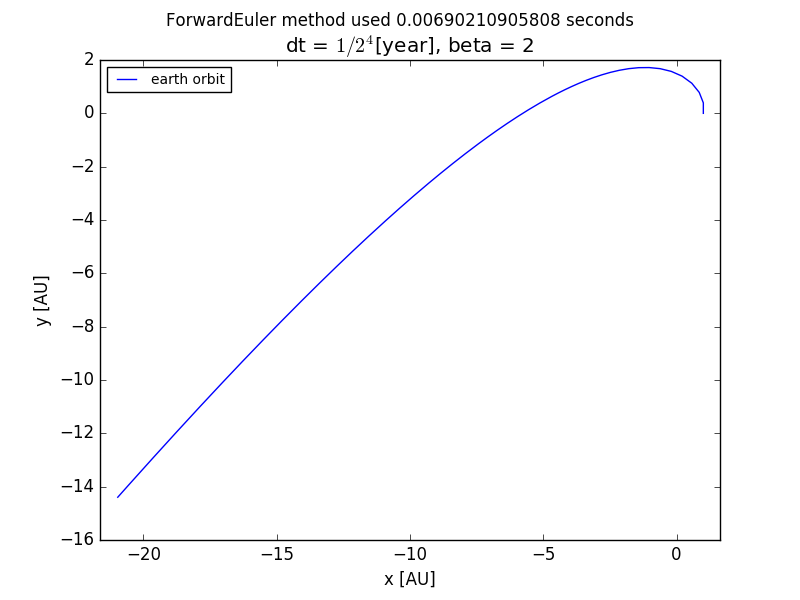
\includegraphics[width=0.70\textwidth]{test_algorithms/stability_test_k4beta200ForwardEuler.png}

\caption{Earth orbit around the sun using the Forward Euler method with $dt = \frac{1}{2^4}$}
\label{fig:Earth_orbit_sun_Forward_Euler_k_4}
\end{figure}
\FloatBarrier


\FloatBarrier
\begin{figure}[!ht]
\centering
\FloatBarrier
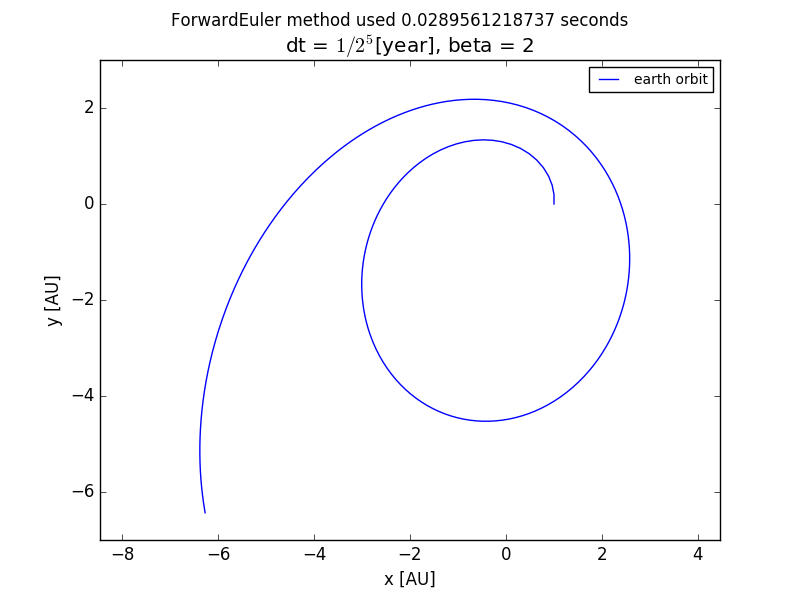
\includegraphics[width=0.70\textwidth]{test_algorithms/stability_test_k5beta200ForwardEuler.png}

\caption{Earth orbit around the sun using the Forward Euler method with $dt = \frac{1}{2^5}$}
\label{fig:Earth_orbit_sun_Forward_Euler_k_5}
\end{figure}
\FloatBarrier


\FloatBarrier
\begin{figure}[!ht]
\centering
\FloatBarrier
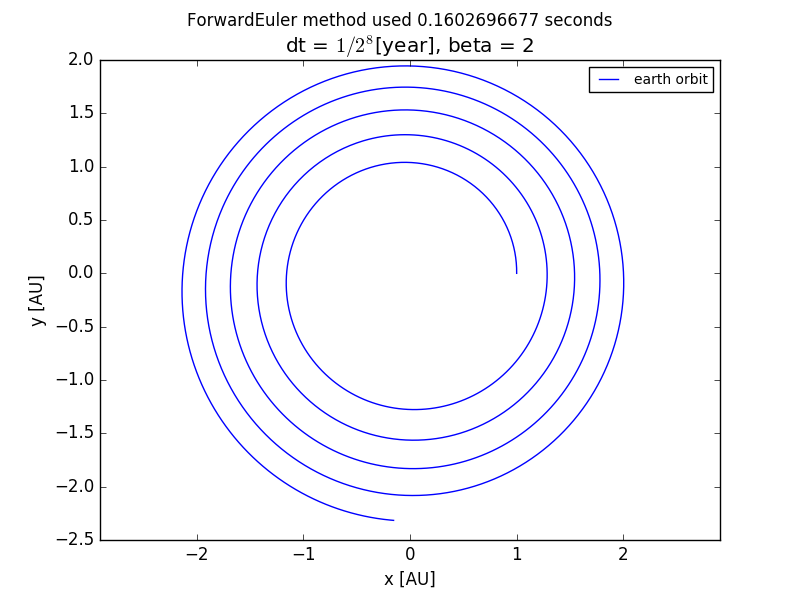
\includegraphics[width=0.70\textwidth]{test_algorithms/stability_test_k8beta200ForwardEuler.png}

\caption{Earth orbit around the sun using the Forward Euler method with $dt = \frac{1}{2^8}$}
\label{fig:Earth_orbit_sun_Forward_Euler_k_8}
\end{figure}
\FloatBarrier


\FloatBarrier
\begin{figure}[!ht]
\centering
\FloatBarrier
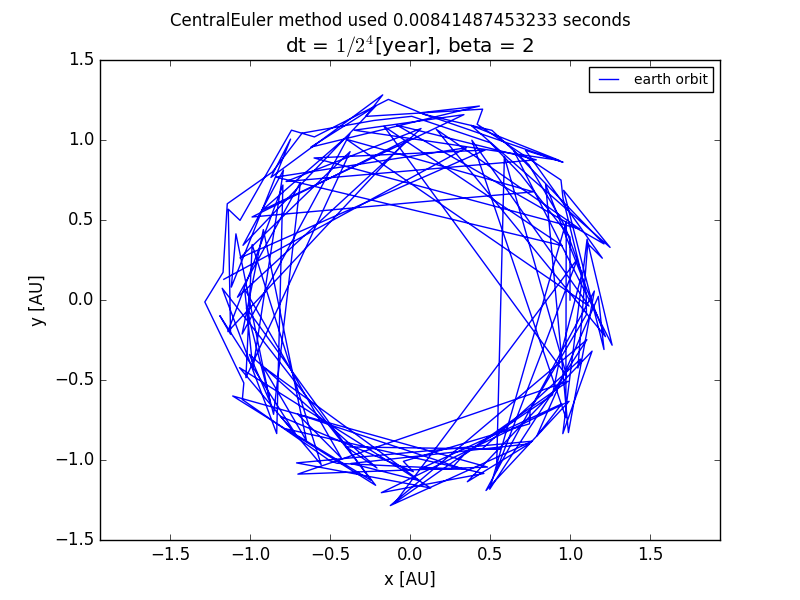
\includegraphics[width=0.70\textwidth]{test_algorithms/stability_test_k4beta200CentralEuler.png}

\caption{Earth orbit around the sun using the Central Euler method with $dt = \frac{1}{2^4}$}
\label{fig:Earth_orbit_sun_Forward_Euler_k_8}
\end{figure}
\FloatBarrier


\FloatBarrier
\begin{figure}[!ht]
\centering
\FloatBarrier
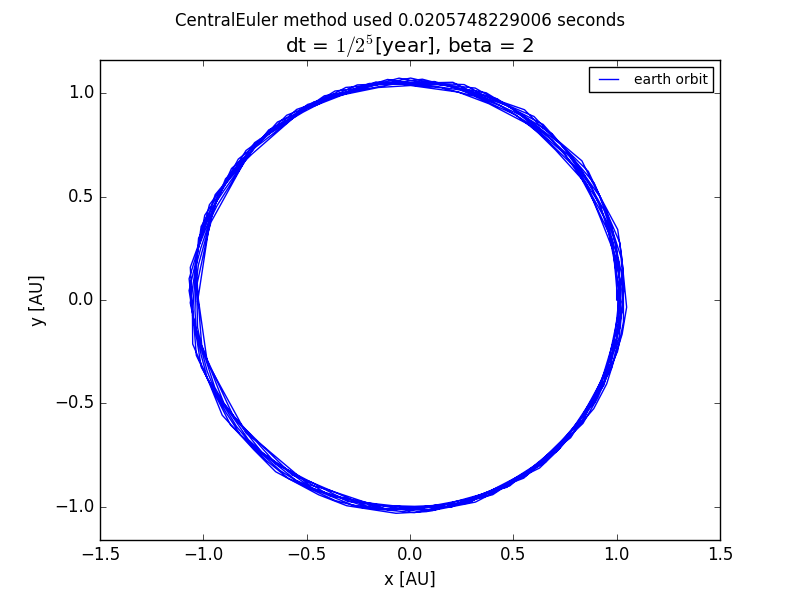
\includegraphics[width=0.70\textwidth]{test_algorithms/stability_test_k5beta200CentralEuler.png}

\caption{Earth orbit around the sun using the Central Euler method with $dt = \frac{1}{2^5}$}
\label{fig:Earth_orbit_sun_Forward_Euler_k_8}
\end{figure}
\FloatBarrier

\FloatBarrier
\begin{figure}[!ht]
\centering
\FloatBarrier
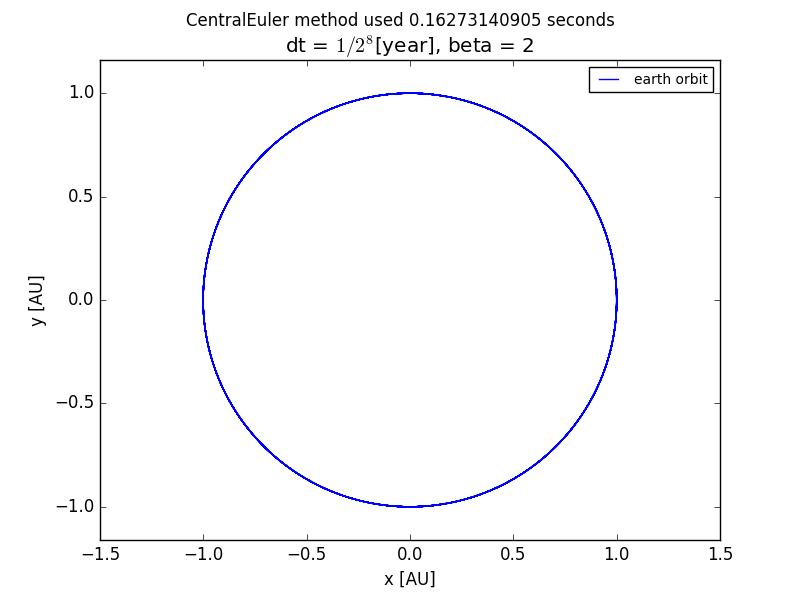
\includegraphics[width=0.70\textwidth]{test_algorithms/stability_test_k8beta200CentralEuler.png}

\caption{Earth orbit around the sun using the Central Euler method with $dt = \frac{1}{2^8}$}
\label{fig:Earth_orbit_sun_Forward_Euler_k_8}
\end{figure}
\FloatBarrier


\FloatBarrier
\begin{figure}[!ht]
\centering
\FloatBarrier
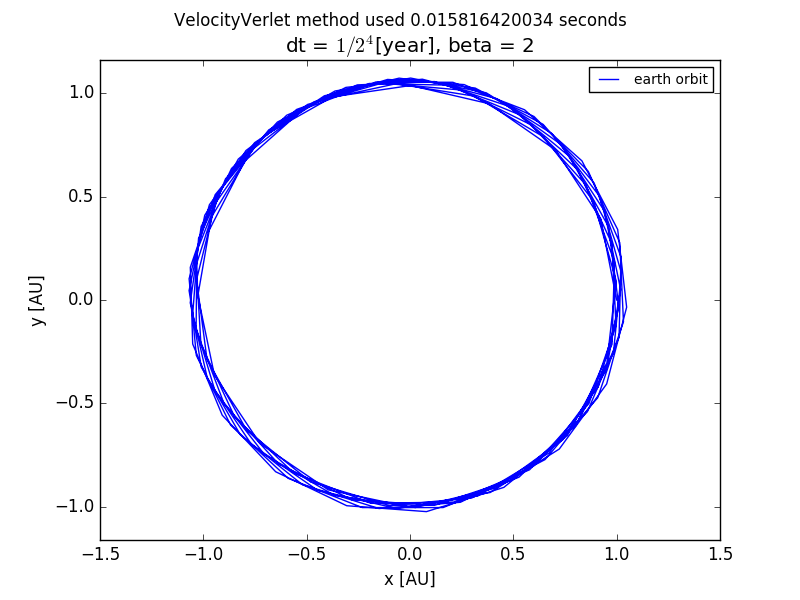
\includegraphics[width=0.70\textwidth]{test_algorithms/stability_test_k4beta200VelocityVerlet.png}

\caption{Earth orbit around the sun using the Velocity Verlet method with $dt = \frac{1}{2^4}$}
\label{fig:Earth_orbit_sun_Forward_Euler_k_8}
\end{figure}
\FloatBarrier



\FloatBarrier
\begin{figure}[!ht]
\centering
\FloatBarrier
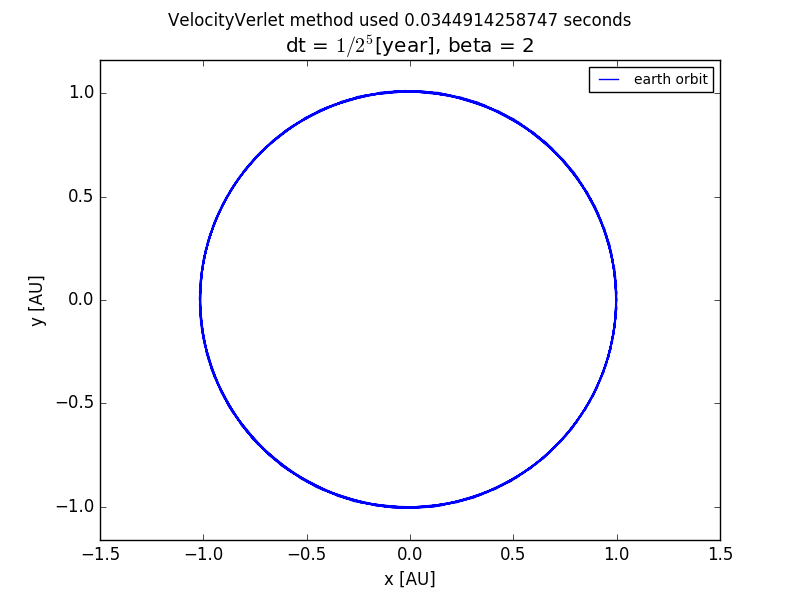
\includegraphics[width=0.70\textwidth]{test_algorithms/stability_test_k5beta200VelocityVerlet.png}

\caption{Earth orbit around the sun using the Velocity Verlet method with $dt = \frac{1}{2^5}$}
\label{fig:Earth_orbit_sun_Forward_Euler_k_8}
\end{figure}
\FloatBarrier


\FloatBarrier
\begin{figure}[!ht]
\centering
\FloatBarrier
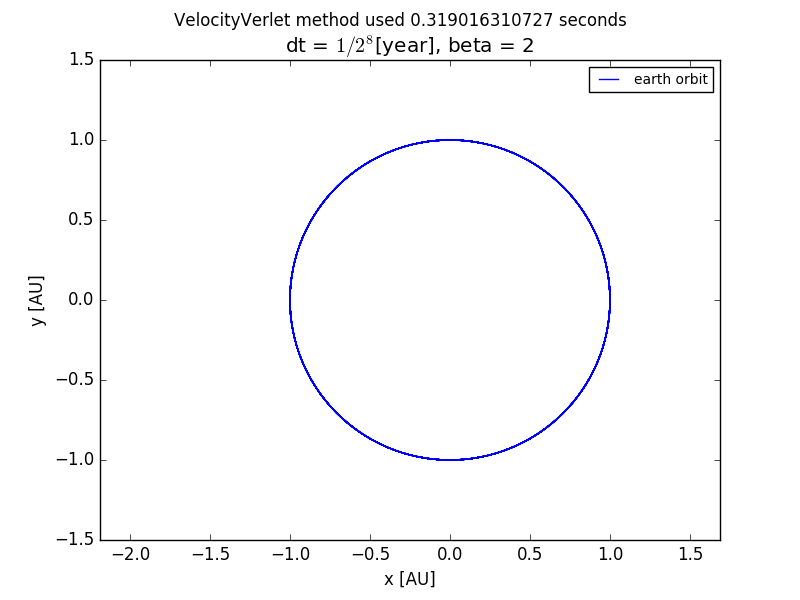
\includegraphics[width=0.70\textwidth]{test_algorithms/stability_test_k8beta200VelocityVerlet.png}

\caption{Earth orbit around the sun using the Velocity Verlet method with $dt = \frac{1}{2^8}$}
\label{fig:Earth_orbit_sun_Forward_Euler_k_8}
\end{figure}
\FloatBarrier


\subsubsection{Conservation of kinetic and potential energies and angular momentum}
Angular momentum for a body in motion under a central force F is defined as follows:\\
$\frac{dL}{dt}=r \times F$\\
, where L is the angular momentum, r is the radius and F is the central force. For a circular orbit, we must assume that the central force and the radius are parallel, which gives a change of angular momentum with respect to time being 0. Therefore the angular momentum must be conserved for circular motion. \\
\\
$E_p = -GM/r$\\
$E_k = 1/2mv^2$\\,
\\
$E_{tot} = constant$\\

Since the radius with respect to time is not changing as well, we have that both the kinetic energy and the potential energy must remain constant.

Now checking for a circular orbits, that the angular momentum, kinetic and potential energies are conserved:\\

For every position we have the velocities. These are decomposed in each direction, x, y and z. The total velocity squared is the sum of the squared velocities in each direction. This is directly linked to kinetic energy. Large maximum differences of the velocities squared for each method, indicates unstable solutions.\\

Low standard deviation for L(angular momentum), $E_k$(kinetic energy ~$v^2$) and $E_p$(potential energy ~$1/r$) would mean that the system is stable. \\

For both CentralEuler and VelocityVerlet, the solutions are decent, with the Velocity Verlet being the most stable. The ForwardEuler is the most unstable, also shown by figures 1, 2 and 3, showing that this method does not approximate an orbit, even when the two other methods do. \\

True values are shown in Table ~\ref{tab:Stability_methods_tabular}\\

\FloatBarrier
\begin{table}
\begin{tabular}{llrrr}
\toprule 
Metric & Unit & Forward Euler & Central Euler & Velocity Verlet \\ 
\midrule 
max diff($v^2$) & $[AU^2/Yr^2]$  & 0.08430  & 0.02381 & 0.00029 \\ 
std($v^2$) &$[AU^2/Yr^2]$ & 4.86822 & 0.02656 & 0.00840 \\  
std(L/$M_{earth}$) &$[AU^2/Yr]$ & 1.52866 &  0.00134 & 1.12180e-14 \\ 
std(1/r) & $[1/AU]$ & 0.11873 & 0.00034 & 0.00011 \\ 
\bottomrule
\end{tabular}
\caption{Stability of methods}
\label{tab:Stability_methods_tabular}
\end{table}
\FloatBarrier

\subsubsection{Timing differences between methods and FLOPs}
Floating point operations are as follows:\\
Central Euler has 2 additions and 2 multiplications = 4n flops\\
Forward Euler has 2 additions and 1 multiplication = 3n flops\\
Velocity Verlet has 3 additions and 3 multiplications = 6n flops\\


Table ~\ref{tab:Timing_differences_FLOPS} shows the runtime differences for each method for varying time steps. The Forward Euler was the fastest method, but clearly this was compensated with bad precision. The Central Euler method had much better precision, and was just slightly slower. The VelocityVerlet was the most precise, and also the slowest. The runtimes can be directly linked to the number of flops as calculated above. 

\FloatBarrier
\begin{table}

\begin{tabular}{lrrrr}
\toprule
{} &  k &  CentralEuler &  ForwardEuler &  VelocityVerlet \\
\midrule
0 &  4 &      0.022213 &      0.019871 &        0.048964 \\
1 &  5 &      0.065837 &      0.048205 &        0.128394 \\
2 &  6 &      0.109570 &      0.101608 &        0.188569 \\
3 &  7 &      0.267016 &      0.214553 &        0.437121 \\
4 &  8 &      0.404209 &      0.396895 &        0.856961 \\
\bottomrule

\end{tabular}

\caption{Runtime in seconds for different sampling time dt. $dt = 1/(2^k)$}
\label{tab:Timing_differences_FLOPS}
\end{table}
\FloatBarrier

%*Code/Implementations/test: Readability of code, implementation, testing and discussion of benchmarks. Total number of possible points 20*

 

\section{Results}
%*Analysis: of results and the effectiveness of their selection and presentation. Are the results well understood and discussed? Total number of possible points: 20*



\subsection{Escape velocities}
\subsubsection{Analytic solution}
Analytically the escape velocity should occur when the kinetic energy is great enough for the object to escape the gravitational force. We have that:\\

$v_{crit} = E_k>E_p$\\

$\frac{M_{earth}v^2}{2} = \frac{GM_{\odot}M_{earth}}{r}$\\

$\implies v_{crit}=\sqrt{\frac{2M_{\odot}G}{r}}$\\

using $GM_{\odot} = 4\pi^2 [AU^3/Yr^2]$\\

$v_{crit} = 2\sqrt{2}\pi [AU/yr]$\\

This means that analytically an initial velocity larger than $2\sqrt{2}\pi [AU/yr]$ would result in the Earth escaping from the sun.\\

\subsubsection{Numerical solution}
If the initial velocity is smaller than $2\pi$ I get the figure ~\ref{fig:Earth_sun_jupiter_v0_pi} showing that small velocities also do not result a circular orbit:

\FloatBarrier
\begin{figure}[!ht]
\centering
\FloatBarrier
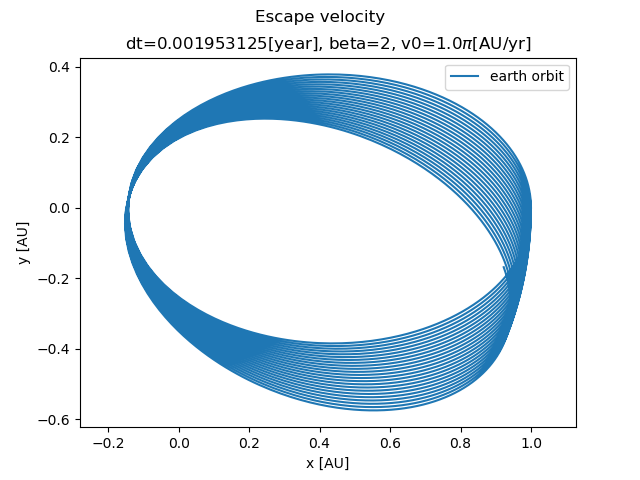
\includegraphics[width=0.70\textwidth]{test_algorithms/escape_velocity_test_k9beta200v010VelocityVerlet.png}

\caption{Initial velocity = $\pi$ [AU/Yr]}
\label{fig:Earth_sun_jupiter_v0_pi}
\end{figure}
\FloatBarrier

Figure ~\ref{fig:Earth_sun_jupiter_v0_2.6_pi} shows that an initial velocity of 2.6$\pi$ gives an elliptical orbit, since we are not at escape velocities.

\FloatBarrier
\begin{figure}[!ht]
\centering
\FloatBarrier
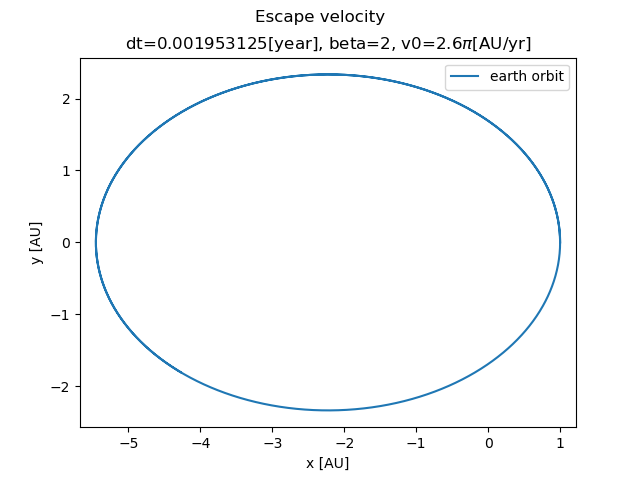
\includegraphics[width=0.70\textwidth]{test_algorithms/escape_velocity_test_k9beta200v026VelocityVerlet.png}

\caption{Initial velocity = $2.6\pi$ [AU/Yr]}
\label{fig:Earth_sun_jupiter_v0_2.6_pi}
\end{figure}
\FloatBarrier

Figure ~\ref{fig:Earth_sun_jupiter_v0_3.0_pi} shows that an initial velocity of 3.0$\pi$ escapes the sun.

\FloatBarrier
\begin{figure}[!ht]
\centering
\FloatBarrier
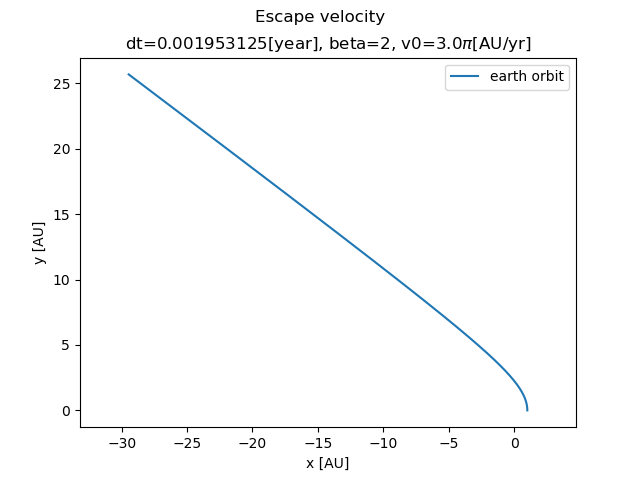
\includegraphics[width=0.70\textwidth]{test_algorithms/escape_velocity_test_k9beta200v030VelocityVerlet.png}

\caption{Initial velocity = $3.0\pi$ [AU/Yr]}
\label{fig:Earth_sun_jupiter_v0_3.0_pi}
\end{figure}
\FloatBarrier

\subsubsection{Varying beta values}

Increasing the beta value means reducing the gravitational force. Figure ~\ref{fig:Earth_sun_jupiter_beta_230_v0_2.0_pi}, ~\ref{fig:Earth_sun_jupiter_beta_270_v0_2.0_pi} and ~\ref{fig:Earth_sun_jupiter_beta_300_v0_2.0_pi} shows that a higher beta value results in a larger radius for the orbit. When beta approaches 3 the orbit of the Earth will spiral out and escape the sun.

\FloatBarrier
\begin{figure}[!ht]
\centering
\FloatBarrier
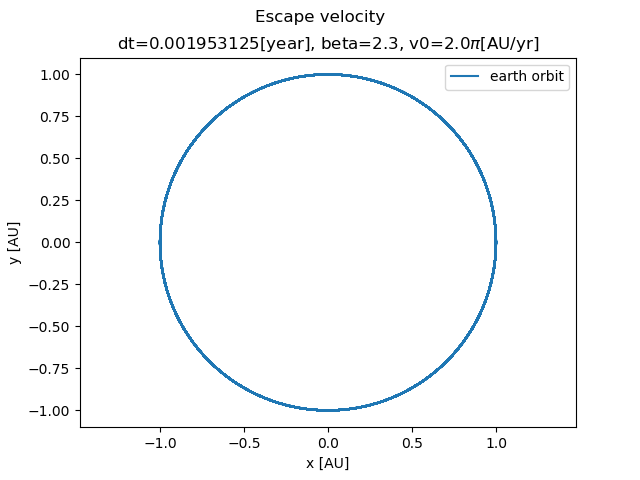
\includegraphics[width=0.70\textwidth]{test_algorithms/escape_velocity_test_k9beta230v020VelocityVerlet.png}

\caption{Initial velocity = $2.0\pi$ and beta = 2.3 [AU/Yr]}
\label{fig:Earth_sun_jupiter_beta_230_v0_2.0_pi}
\end{figure}
\FloatBarrier

\FloatBarrier
\begin{figure}[!ht]
\centering
\FloatBarrier
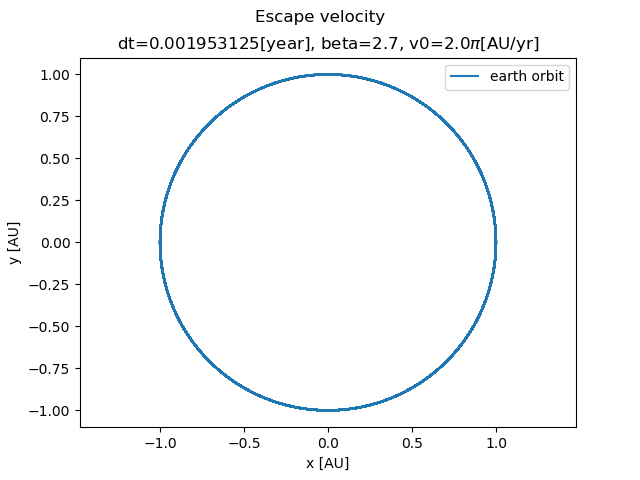
\includegraphics[width=0.70\textwidth]{test_algorithms/escape_velocity_test_k9beta270v020VelocityVerlet.png}

\caption{Initial velocity = $2.0\pi$ and beta = 2.7 [AU/Yr]}
\label{fig:Earth_sun_jupiter_beta_270_v0_2.0_pi}
\end{figure}
\FloatBarrier

\FloatBarrier
\begin{figure}[!ht]
\centering
\FloatBarrier
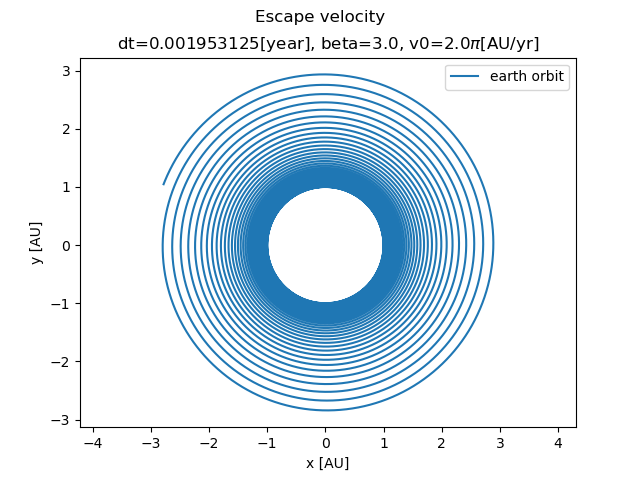
\includegraphics[width=0.70\textwidth]{test_algorithms/escape_velocity_test_k9beta300v020VelocityVerlet.png}

\caption{Initial velocity = $2.0\pi$ and beta = 3.0 [AU/Yr]}
\label{fig:Earth_sun_jupiter_beta_300_v0_2.0_pi}
\end{figure}
\FloatBarrier


\subsection{3-body-problem}

\FloatBarrier
\begin{figure}[!ht]
\centering
\FloatBarrier
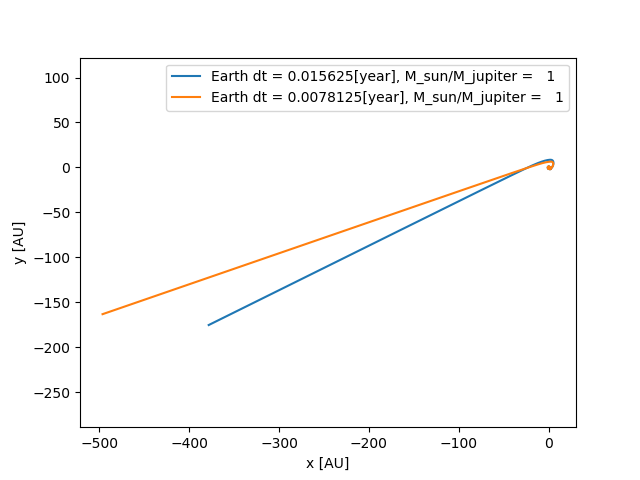
\includegraphics[width=0.70\textwidth]{test_three_body_problem/stability_2d_test_k70beta200VelocityVerlet.png}

\caption{The difference in discretization shows how vital the differences can be}
\label{fig:Earth_orbit_sun_Forward_Euler_k_8}
\end{figure}
\FloatBarrier

Figure ~\ref{fig:Earth_jupiter} shows the Earth, Sun and Jupiter in one plot.

\FloatBarrier
\begin{figure}[!ht]
\centering
\FloatBarrier
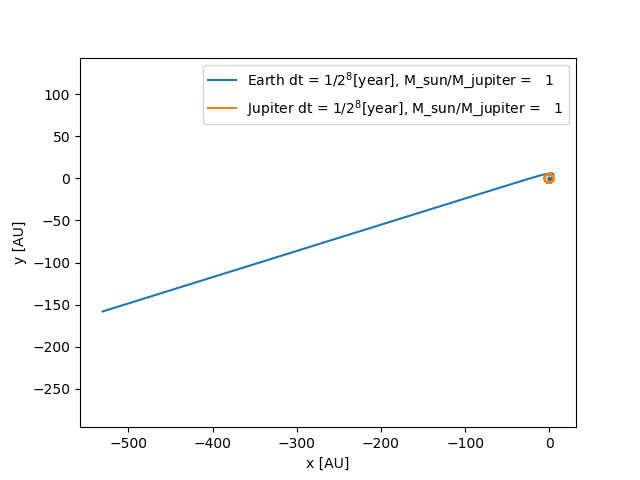
\includegraphics[width=0.70\textwidth]{final_model/stability_2d_test_k8beta200VelocityVerlet.png}

\caption{Earth, Sun and Jupiter in one plot}
\label{fig:Earth_jupiter}
\end{figure}
\FloatBarrier



\subsection{Final Model}
Below is a final plot of the solar system:\\

\FloatBarrier
\begin{figure}[!ht]
\centering
\FloatBarrier
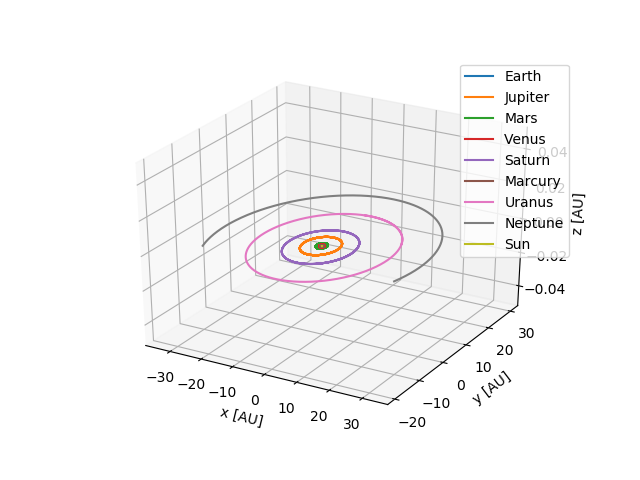
\includegraphics[width=0.70\textwidth]{final_model/stability_3d_test_k8beta200VelocityVerlet.png}

\caption{Final model of the solar system}
\label{fig:Earth_orbit_sun_Forward_Euler_k_8}
\end{figure}
\FloatBarrier




\subsection{The perihelion precession of Mercury}
I was not able to finish the general relativity problem trying to figure out if the observed perihelion precession of Mercury quite in time, but I have given a link to the program I have made here:
$\href{https://github.com/larsjbro/FYS4150/blob/master/Project_3/source/test_perihelion/test_perihelion.py}{https://github.com/larsjbro/FYS4150/blob/master/Project_3/source/test_perihelion/test_perihelion.py}$
 


\section{Conclusion}
To start with the test for numerical method of choice showed that the Velocity Verlet method was the best of the three. I could see that the method of choice plays a huge role in the search for reliable results. Also I found that the runtimes depended very much on number of floating point operations. Nevertheless the precision needs to be at a minimum regardless of speed. The sun is huge, and it took a lot of effort to neutralize the gravitational force\\


%*Conclusions, discussions and critical comments: on what was learned about the method used and on the results obtained. Possible directions and future improvements? Total number of possible points: 10*




\section{References}
\subsection{Internet sources}

-$\href{https://github.com/CompPhysics/ComputationalPhysics/blob/gh-pages/doc/Lectures/lectures2015.pdf}{https://github.com/CompPhysics/ComputationalPhysics/blob/gh-pages/doc/Lectures/lectures2015.pdf}$, October 2017\\

$\href{https://ssd.jpl.nasa.gov/horizons.cgi}{https://ssd.jpl.nasa.gov/horizons.cgi}$, NASA, October 2017, used to generate ephemerides\\




%\FloatBarrier
%\begin{figure}[!ht]
%\centering
%\FloatBarrier
%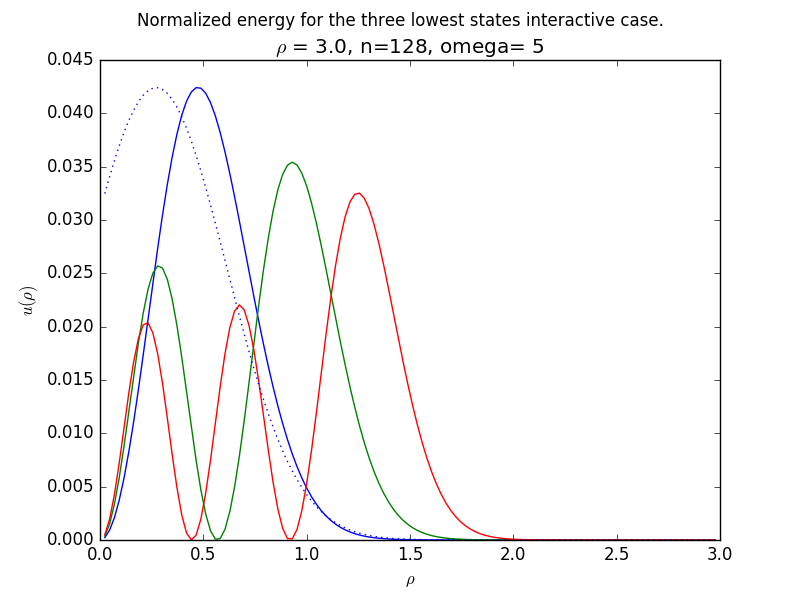
\includegraphics[width=0.45\textwidth]{eigenvector_rho29n128omega500.png}
%
%\caption{Normalized energy for the three lowest eigenvalues for repulsive Coulomb interaction with n=128 and $\omega_r$=5}
%\label{fig:Eigenvalue_states_n_320_omega_500}
%\end{figure}
%\FloatBarrier


